\documentclass[a4paper]{scrartcl}
\usepackage[utf8]{inputenc}
\usepackage[english]{babel}
\usepackage{graphicx}
\usepackage{lastpage}
\usepackage{pgf}
\usepackage{wrapfig}
\usepackage{fancyvrb}
\usepackage{fancyhdr}
\pagestyle{fancy}

% Create header and footer
\headheight 27pt
\pagestyle{fancyplain}
\lhead{\footnotesize{Internet Applications, ID1354}}
\chead{\footnotesize{Name of the Report}}
\rhead{}
\lfoot{}
\cfoot{\thepage\ (\pageref{LastPage})}
\rfoot{}

% Create title page
\title{Name of the Report}
\subtitle{Internet Applications, ID1354}
\author{Your Name and Email Address}
\date{Date}

\begin{document}

\maketitle

\section*{Tips for Report Writing}
\textbf{REMOVE THIS SECTION BEFORE SUBMITTING THE REPORT.}\\

\noindent \textit{The target audience has exactly the same skills as the author, except they do not know anything at all about the specific program described in the report.} \\

Consider the following:

\begin{itemize}
  \item \textbf{The report must be \textit{centered around the requirements}. Which are they (Introduction), how did you work to meet them (Method), what is the solution that meets them (Result), and how can you be sure they are met (Discussion). This is the IMRaD method.}

  \item \textbf{The report must show that you have done the work yourself and that you have understood what you have done. Both of these goals are met by carefully explaining the source code.}

  \item Is spelling and grammar correct? Is spoken language avoided?

  \item Does the report have a good structure with sections, subsections and paragraphs?

  \item Is the solution clearly explained? Will the reader understand the program? What would you yourself want to know if you read about the program, is that included in the report?

  \item Is the solution analyzed and evaluated? Are important properties of the program explained? Should there have been more extensive evaluation?

  \item Is the text clarified with images and/or other figures, and with links to the code in your Git repository? Remember that all figures (images, tables, graphs, code listings, etc) shall be numbered and have a short explaining text.
\end{itemize}

\section{Introduction}

This assignment focuses on learning PHP for server-side programming. The knowledge will be applied to the website created in the first assignment to expand its functionality. The acquired PHP knowledge is tested by a set of requirements that can be divided into two parts. The first part is authentication and includes the following requirements.
\begin{itemize}
    \item Provide a log in form on the website using HTML and CSS that matches the style of the website.
    \item Each user is associated with a name and a password that is stored on the server.
    \item The action of the html attribute can not be set to a PHP function but instead a URL.
    \item The login must follow the five basic heuristics for user interface design. 
\end{itemize}

The second part concerns commenting on the recipes located on the website. The comments have previously been hard-coded in HTML which will now be changed. The requirements for this part are summarised as follows.
\begin{itemize}
    \item Logged in users should be able to leave comments on the recipes.
    \item The comments should be displayed on the relevant recipe page.
    \item All users should be able to read all comments.
    \item Comments and their author should be stored permanently on the server.
    \item Logged in users should be able to delete their own comments, which needs to be verified server-side.
    \item Commenting mys follow the five basic heuristics for user interface design.
\end{itemize}

\textbf{This section tells \textit{what} are you going to do.} \\

\noindent Explain the task and the requirements on the solution. It is very important to \textit{clearly state the requirements}. If you wrote the program together with other students, list their names and email addresses here.

\section{Literature Study}

During the last assignment a simple http server server [XXX] was used which is quick and easy to set up but very limited. To finish this assignment a complete LAMP stack will be used running on Arch Linux. A good resource to set up the LAMP stack on Arch can be found at [XXX]. Since a database is used for the server-side storage of information of the comments, [XXX] seems like a good resource for implementation-specific information for this type of a system. It includes information about creating comments, saving them to a database and also deleting existing comments. 


This section must prove that you collected sufficient knowledge before starting development, instead of just hacking away without knowing how to complete the task. State what you have read and briefly summarize what you have learned.

\section{Method}

The LAMP stack was installed on a Linux machine running the Arch distrobution. The web server is Apache 2.4.37 and the specific MySQL implementation is MariaDB which is made by the original developers of MySQL. The PHP version number is 7.2.12 and DBeaver is being used as a database tool for easier setup of the database.

\textbf{This section tells \textit{how} you solved the task.} \\

\noindent Explain how you worked when solving the tasks and how you evaluated that your solution met the requirements. Mention development tools and IDEs you used. \textit{Do not explain your solution and do not refer to code}, that belongs to the \textit{Result} section.

\section{Result}

The login form was put on a separate page with a link in the navbar that is visible from all other pages on the site. The login page is seen in figure \ref{fig:login_form} and the link in the navigation bar can also be seen in the upper right corner. When a user logs in a query is sent to the database to match the username and password to rows in a table called Users. If there is a match the user is logged in and the username is saved in the PHP session variable. 

\begin{figure}[h!]
  \begin{center}
    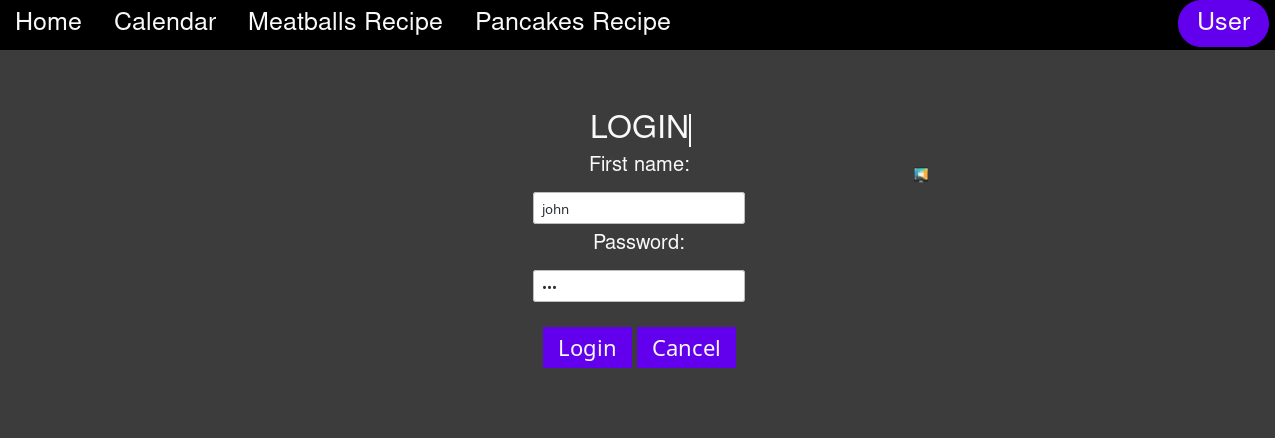
\includegraphics[scale=0.3]{images/login_form.png}
    \caption{A sample user interface screenshot to illustrate caption (this text), numbering and reference in text.}
    \label{fig:login_form}
  \end{center}
\end{figure}

\textbf{This section explains \textit{the result} of what you did.} \\

\noindent Present the solution. Explain your code and prove that it meets the requirements. It is very important to \textit{state each requirement that is met} and explain \textit{how you met it}. It is also important to include links to your code in your Git repository, user interface screen-shots, see Figure \ref{fig:ui}, and other figures to illustrate your reasoning. Also remember that these figures must be referenced in the text.

\section{Discussion}

\textbf{This section \textit{analysis} the result presented in the previous section.} \\

\noindent Summarize the requirements and \textit{clearly state which of them you have met}. What lessons have you learned and what problems did you face? How were the problems solved? Should you have done something differently?

\section{Comments About the Course}

Any comment(s) related to this course offering or to coming offerings is much appreciated. \textit{Please also tell approximately how much time you spent on the assignment}, including lectures and exercises. This is of great help for course evaluation.

\end{document}
